\chapter{Carboxylic Acid Derivatives}\label{ch:b2:acyl-substitution}

Boil olive oil with sodium hydroxide and you get soap and glycerol: the
oldest organic reaction run on purpose. The oil is an ester of glycerol and
long-chain acids, and the hydroxide cuts each ester at one bond, always the
same one, between the carbonyl carbon and the oxygen of the alcohol. Esters,
acids, amides, anhydrides and \omterm{def:b2:acyl-substitution:derivative}{acyl chlorides} all react in this way: a
nucleophile adds to the carbonyl carbon, and a group leaves. Ranking these
compounds by how well their group leaves tells which can be turned into which,
and in which direction a chemist must go uphill.

\begin{recall}
The Year 1 volume: electrophilic activation of a carbonyl group, the mechanisms of hemiacetal and
acetal formation, organomagnesium additions, hydride donors and their scope, leaving groups,
$\mathrm pK_a$, $Q$ and $K$. \Cref{ch:b2:amines}: \omterm{def:b2:amines:nucleophilic-addition}{nucleophilic addition}, amines.
\Cref{ch:b2:equilibrium-shifts}: shifting an equilibrium. The school volume: esters, carboxylic acids
and amides.
\end{recall}

\begin{omfigure}
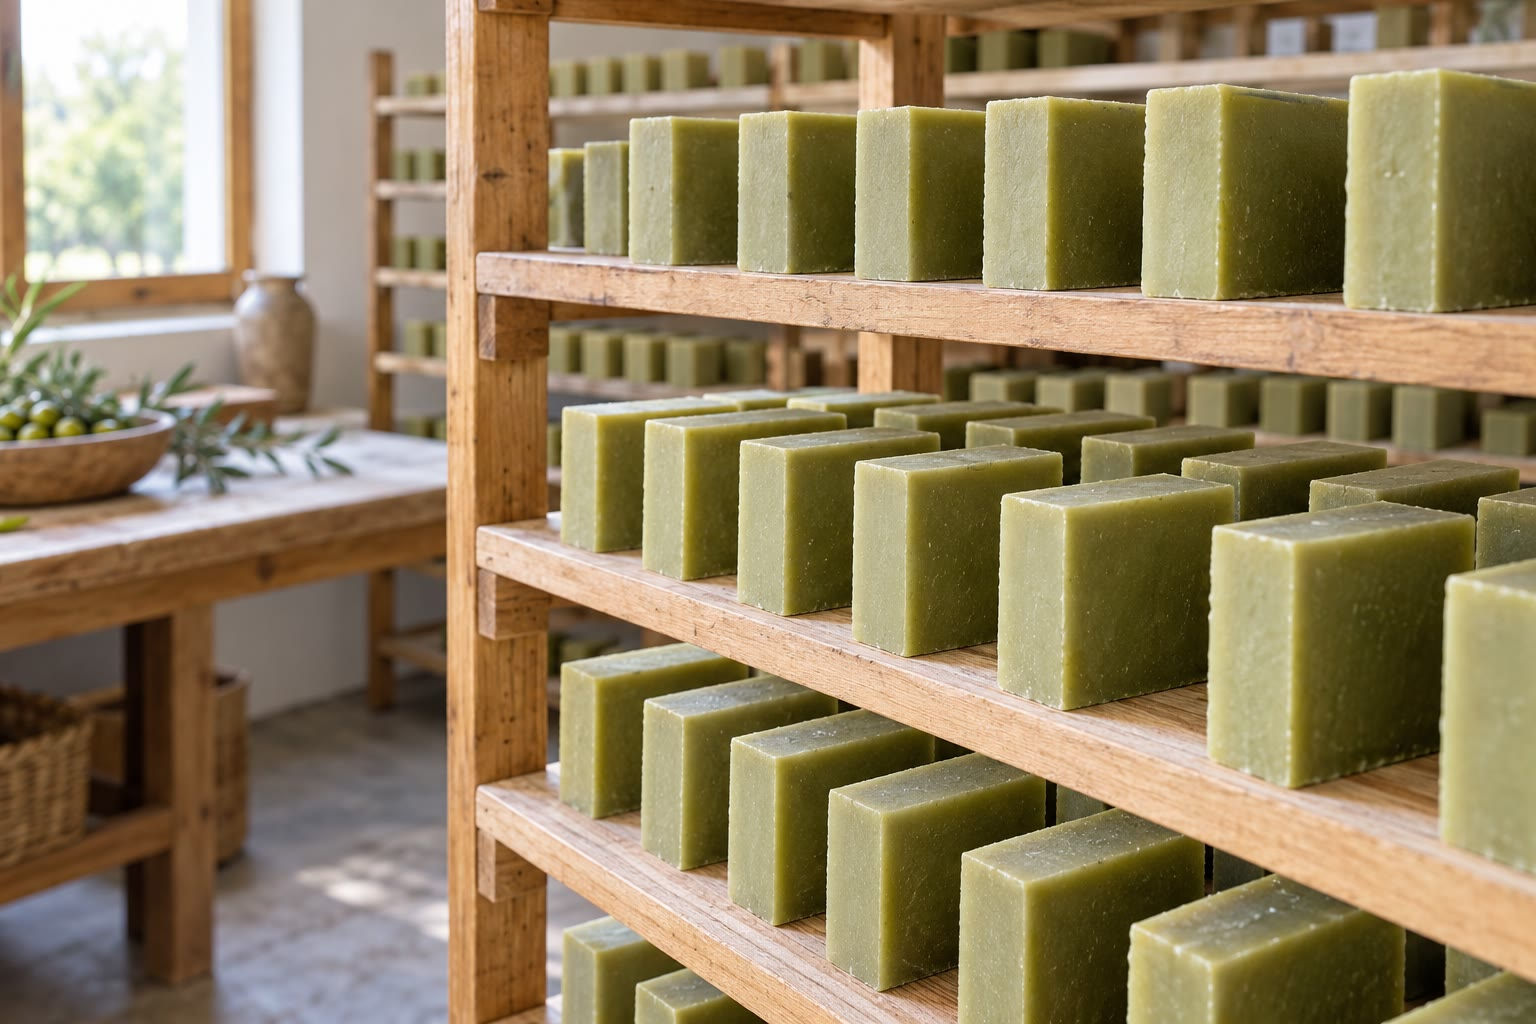
\includegraphics[width=0.58\linewidth]{images/book3/ai/b2-24-soap-bars.jpg}

{\small Bars of olive-oil soap drying on wooden racks. Soap is the sodium salt of the fatty acids
released when the oil, an ester, is boiled with sodium hydroxide.}
\end{omfigure}

\section{The family and its reactivity}

\begin{definition}[Carboxylic acid derivatives]\label{def:b2:acyl-substitution:derivative}
A \emph{carboxylic acid derivative}\index{carboxylic acid derivative} is a compound \ce{R-CO-Z} in
which the \ce{OH} of a carboxylic acid is replaced by another group Z. The \emph{acyl
group}\index{acyl group} $\mathrm{R{-}CO{-}}$ is common to all of them. In an \emph{acyl chloride}\index{acyl
chloride}, Z is Cl; in an \emph{acid anhydride}\index{acid anhydride}, Z is $\mathrm{O{-}CO{-}R'}$, two acyl
groups sharing one oxygen; in an ester Z is $\mathrm{OR'}$, in an amide $\mathrm{NR'_2}$.
\end{definition}

\begin{proposition}[Reactivity scale]\label{prop:b2:acyl-substitution:reactivity}
Towards nucleophiles, the derivatives react in the order \omterm{def:b2:acyl-substitution:derivative}{acyl chloride} $>$ anhydride $>$ ester
$\approx$ acid $>$ amide.
\end{proposition}

\begin{proof}[Argument]
Two effects add up. The leaving group \ce{Z-} leaves the more easily the weaker a base it is:
\ce{Cl-} (conjugate acid \ce{HCl}, $\mathrm pK_a$ about $-7$) much better than a carboxylate
($\mathrm pK_a$ about 5), an alkoxide (about 16) or an amide ion (about 35). And the group Z gives
electron density to the carbonyl by mesomeric donation of its lone pair, which makes the carbonyl
carbon less electrophilic: weak for Cl, strongest for nitrogen. The amide is both the poorest
electrophile and the poorest leaving group.
% ledger: pka:ethanoic, pka:ethanol
\end{proof}

\section{Nucleophilic acyl substitution}

\begin{definition}[Nucleophilic acyl substitution]\label{def:b2:acyl-substitution:nas}
A \emph{nucleophilic acyl substitution}\index{nucleophilic acyl substitution} replaces the group Z
of an acyl compound by a nucleophile. It proceeds by addition of the nucleophile to the carbonyl
carbon, giving a \emph{tetrahedral intermediate}\index{tetrahedral intermediate}, followed by
elimination of the leaving group, which restores the \ce{C=O} bond.
\end{definition}

\begin{proposition}[Addition--elimination]\label{prop:b2:acyl-substitution:addition-elimination}
Acyl substitution goes through a \omterm{def:b2:acyl-substitution:nas}{tetrahedral intermediate}; it is accelerated in base by a stronger
nucleophile and in acid by activation of the carbonyl.
\end{proposition}

\begin{proof}[Argument]
The carbonyl carbon, planar and electrophilic, accepts the nucleophile from above or below its
plane, as in the additions of \cref{ch:b2:amines}; with a group Z able to leave, the intermediate
expels it instead of being protonated. In base the nucleophile is an anion (\ce{HO-},
\ce{RO-}); in acid the carbonyl oxygen is protonated and a neutral nucleophile (water, an alcohol)
suffices. Esters labelled with \ce{^{18}O} in the alcohol part give, on hydrolysis, labelled alcohol
and unlabelled acid: the bond broken is the acyl--oxygen bond, as the mechanism requires.
\end{proof}

\begin{omfigure}
\setchemfig{atom sep=1.7em}
\schemestart
\chemfig{R-C(=[2]O)-OR'} \+ \chemfig{HO^{-}}
\arrow{->[addition]}
\chemfig{R-C(-[2]O^{-})(-[6]OH)-OR'}
\arrow{->[elimination]}[,1.3]
\chemfig{R-C(=[2]O)-OH} \+ \chemfig{^{-}OR'}
\schemestop

\medskip
\schemestart
\chemfig{R-C(=[2]O)-OH} \+ \chemfig{^{-}OR'}
\arrow{->[proton transfer]}
\chemfig{R-C(=[2]O)-O^{-}} \+ \chemfig{HOR'}
\schemestop
\par\vspace{6pt}

{\small \omterm{def:b2:acyl-substitution:saponification}{Saponification} of an ester. Hydroxide adds to the carbonyl carbon, giving the \omterm{def:b2:acyl-substitution:nas}{tetrahedral
intermediate}; the alkoxide leaves and the \ce{C=O} bond reforms; the alkoxide, a strong base, then
takes the proton of the acid. This last step makes the reaction complete.}
\end{omfigure}

\begin{method}[Drawing an acyl substitution]\label{met:b2:acyl-substitution:nas-mechanism}
\begin{enumerate}
  \item In base: the anionic nucleophile adds to the carbonyl carbon; the negative charge goes to
        oxygen; the \ce{C=O} bond reforms and Z leaves; finish with any acid--base step.
  \item In acid: protonate the carbonyl oxygen; the neutral nucleophile adds; transfer a proton
        to the leaving group; it leaves as a neutral molecule; deprotonate the carbonyl.
  \item Count the steps: every intermediate is either tetrahedral or a carbonyl compound.
\end{enumerate}
\end{method}

\section{Esters}

\begin{definition}[Esterification]\label{def:b2:acyl-substitution:esterification}
An \emph{esterification}\index{esterification} forms an ester from a carboxylic acid (or a more
reactive derivative) and an alcohol. The direct reaction of an acid with an alcohol, catalysed by a
strong acid, is the Fischer esterification.
\end{definition}

\begin{proposition}[Fischer esterification]\label{prop:b2:acyl-substitution:fischer}
The Fischer \omterm{def:b2:acyl-substitution:esterification}{esterification} is a slow equilibrium, with a constant near 4 for primary alcohols; it
is driven forward by an excess of one reagent or by removing water as it forms.
\end{proposition}

\begin{proof}[Argument]
Equimolar ethanol and ethanoic acid stop when two thirds of the acid is esterified: $K =
(2/3)^2/(1/3)^2 = 4$. With $Q < K$ maintained by an excess of alcohol, or by distilling water off
(the Dean--Stark trap of the Year 1 volume), the reaction proceeds further
(\cref{ch:b2:equilibrium-shifts}). The six steps of the mechanism are those of \cref{met:b2:acyl-substitution:nas-mechanism}
in acid, all reversible.
% ledger: ester:berthelot
\end{proof}

\begin{definition}[Saponification]\label{def:b2:acyl-substitution:saponification}
A \emph{saponification}\index{saponification} is the hydrolysis of an ester by a hydroxide, giving
the carboxylate salt and the alcohol.
\end{definition}

\begin{proposition}[Saponification is complete]\label{prop:b2:acyl-substitution:saponification}
\omterm{def:b2:acyl-substitution:saponification}{Saponification} goes to completion: its last step, the proton transfer from the carboxylic acid to
the alkoxide, has an equilibrium constant of order $10^{11}$.
\end{proposition}

\begin{proof}
For $\mathrm{RCOOH + R'O^- \to RCOO^- + R'OH}$,
\[
  K = \frac{K_a(\ce{RCOOH})}{K_a(\mathrm{R'OH})} = 10^{\mathrm pK_a(\mathrm{R'OH}) - \mathrm pK_a(\ce{RCOOH})} ;
\]
with ethanoic acid (4.76) and ethanol (15.93), $K = 10^{11.2}$. The carboxylate, a poor electrophile, is not attacked by the alcohol: the overall
reaction does not go back.
% ledger: pka:ethanoic, pka:ethanol
\end{proof}

\begin{omfigure}
\setchemfig{atom sep=1.7em}
\schemestart
\chemfig{CH_2(-[0]O-CO-R)-[6]CH(-[0]O-CO-R)-[6]CH_2-[0]O-CO-R}
\+ \chemfig{3\,NaOH}
\arrow{->[heat]}
\chemfig{CH_2(-[0]OH)-[6]CH(-[0]OH)-[6]CH_2-[0]OH}
\+ \chemfig{3\,R-COO^{-}\,Na^{+}}
\schemestop
\par\vspace{6pt}

{\small \omterm{def:b2:acyl-substitution:saponification}{Saponification} of a triglyceride: the three ester bonds are cut, giving glycerol and
three molecules of the sodium carboxylate, the soap (R a long chain, \ce{C17H33} for the oleate of
olive oil).}
\end{omfigure}

\begin{definition}[Transesterification]\label{def:b2:acyl-substitution:transesterification}
A \emph{transesterification}\index{transesterification} exchanges the alcohol part of an ester,
$\mathrm{RCOOR' + R''OH \rightleftharpoons RCOOR'' + R'OH}$, under acid or base catalysis.
\end{definition}

\begin{definition}[Lactones and lactams]\label{def:b2:acyl-substitution:lactone}
A \emph{lactone}\index{lactone} is a cyclic ester, formed by internal \omterm{def:b2:acyl-substitution:esterification}{esterification} of a
hydroxy acid; a \emph{lactam}\index{lactam} is a cyclic amide.
\end{definition}

\section{Activated derivatives}

Going down the reactivity scale is easy: an \omterm{def:b2:acyl-substitution:derivative}{acyl chloride} gives an anhydride, an ester or an
amide with the right nucleophile, often at room temperature. Going up needs activation: a
carboxylic acid is turned into its chloride by thionyl chloride,
\[
  \ce{RCOOH + SOCl2 -> RCOCl + SO2 + HCl} ,
\]
whose by-products are gases. The \omterm{def:b2:acyl-substitution:derivative}{acyl chloride} then reacts with an alcohol or an amine; a base
(pyridine, triethylamine, or a second equivalent of the amine) traps the \ce{HCl} formed, which
would otherwise protonate the amine.

\begin{method}[Moving along the derivatives]\label{met:b2:acyl-substitution:ladder}
\begin{enumerate}
  \item Down the scale (chloride $\to$ anhydride $\to$ ester, acid $\to$ amide): treat with the
        nucleophile, with a base to take up the acid released.
  \item Up the scale: convert the acid into the chloride first (\ce{SOCl2}); an ester or amide is
        first hydrolysed to the acid.
  \item Between an acid and an ester: Fischer \omterm{def:b2:acyl-substitution:esterification}{esterification} (equilibrium) or \omterm{def:b2:acyl-substitution:saponification}{saponification}
        (complete) followed by acidification.
\end{enumerate}
\end{method}

\begin{omfigure}
\begin{tikzpicture}[font=\small, >={Stealth}]
  \foreach \y/\n in {4/{acyl chloride \ce{RCOCl}}, 3/{anhydride \ce{(RCO)2O}}, 2/{ester $\mathrm{RCOOR'}$ \quad acid \ce{RCOOH}}, 1/{amide $\mathrm{RCONR'_2}$}} {
    \node[cyclenode, minimum width=5.2cm] at (0,\y*1.1) {\n};
  }
  \draw[->, thick, omDef] (-3.1,4.3) -- (-3.1,1.1) node[midway, left, align=right, font=\scriptsize] {easy:\\ nucleophile\\ + base};
  \draw[->, thick, omThm] (3.1,2.2) -- (3.1,4.4) node[midway, right, align=left, font=\scriptsize] {uphill:\\ via the acid\\ and \ce{SOCl2}};
  \node[font=\scriptsize, anchor=south] at (0,4.85) {more reactive};
  \node[font=\scriptsize, anchor=north] at (0,0.55) {less reactive};
\end{tikzpicture}

{\small The reactivity ladder of \omterm{def:b2:acyl-substitution:derivative}{carboxylic acid derivatives}. Any derivative can be turned into
one below it by a nucleophile; climbing goes through the acid and its chloride.}
\end{omfigure}

\section{Organometallics and hydrides}

\begin{proposition}[Two Grignard additions]\label{prop:b2:acyl-substitution:grignard-ester}
An ester treated with excess organomagnesium reagent gives a tertiary alcohol bearing two
identical groups from the reagent.
\end{proposition}

\begin{proof}[Argument]
The first addition gives a \omterm{def:b2:acyl-substitution:nas}{tetrahedral intermediate} that expels the alkoxide: a ketone. A ketone
is more electrophilic than an ester (no mesomeric donation from an $\mathrm{OR'}$ group) and reacts with
the reagent faster than the remaining ester; the second addition, to the ketone, gives the alkoxide
of a tertiary alcohol, which acid work-up protonates. The reaction cannot be stopped at the ketone.
\end{proof}

\begin{proposition}[Hydride reductions]\label{prop:b2:acyl-substitution:hydrides}
Lithium aluminium hydride reduces esters and acids to primary alcohols, and amides to amines;
sodium borohydride reduces aldehydes and ketones but not esters, acids or amides. A bulky aluminium
hydride (DIBAL-H) at \qty{-78}{\degreeCelsius} reduces an ester to the aldehyde.
\end{proposition}

\begin{proof}[Argument]
\ce{LiAlH4} is a strong hydride donor: like the Grignard reagent it adds twice to an ester (through
the aldehyde). Borohydride is too weak for the less electrophilic ester carbonyl. With DIBAL-H at
low temperature the \omterm{def:b2:acyl-substitution:nas}{tetrahedral intermediate}, held by aluminium, does not expel the alkoxide until
the aqueous work-up, when no hydride is left: the aldehyde survives. In an amide, the oxygen,
bound to aluminium, is eliminated instead of the nitrogen, leaving an iminium ion that the hydride
reduces to the amine.
\end{proof}

\begin{history}[Chevreul and the fats]
\begin{minipage}[t]{0.22\linewidth}
\vspace{0pt}
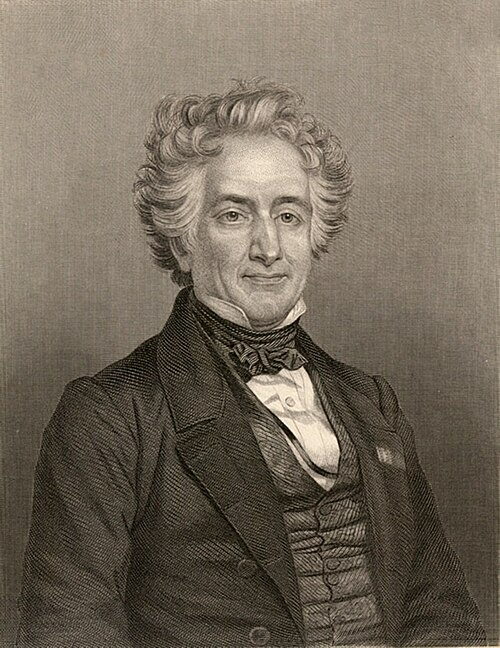
\includegraphics[width=\linewidth]{images/book3/chevreul.jpg}
\end{minipage}\hfill
\begin{minipage}[t]{0.74\linewidth}
\vspace{0pt}
Michel Eugène Chevreul showed, in a study published in 1823, that fats are compounds of glycerol
with fatty acids, which he isolated and named (stearic, oleic, butyric acids), and that
\omterm{def:b2:acyl-substitution:saponification}{saponification} splits them into these two parts. His work turned soap- and candle-making into
chemistry; he lived to be 102. (Portrait by Nicolas Eustache Maurin, public domain, Wikimedia
Commons.)
\end{minipage}
\end{history}

\begin{safety}{\ghs[5mm]{GHS02}\,\ghs[5mm]{GHS05}\,\ghs[5mm]{GHS06}}
Thionyl chloride and \omterm{def:b2:acyl-substitution:derivative}{acyl chlorides} react violently with water and release corrosive gases; they
are handled dry, in a fume hood. Lithium aluminium hydride ignites in contact with water; its
excess is destroyed carefully at the end. Concentrated sodium hydroxide is corrosive to skin and
eyes. Methanol is toxic and flammable.
% ledger: ghs:SOCl2, ghs:ethanoyl-chloride, ghs:LiAlH4, ghs:NaOH, ghs:methanol
\end{safety}

\section{Exercises}

\begin{exercise}[$\star$]\label{exo:b2:acyl-substitution:1}
Rank by reactivity towards water: ethyl ethanoate, ethanoyl chloride, ethanamide, ethanoic
anhydride.
\end{exercise}

\begin{exercise}[$\star$]\label{exo:b2:acyl-substitution:2}
Give the products of ethanoyl chloride with: water; ethanol; ammonia (2 equivalents);
sodium ethanoate; dimethylamine with triethylamine.
\end{exercise}

\begin{exercise}[$\star$]\label{exo:b2:acyl-substitution:3}
Write the \omterm{def:b2:acyl-substitution:saponification}{saponification} of methyl benzoate by sodium hydroxide and compute the mass of sodium
hydroxide needed for \qty{13.6}{g} of the ester.
\end{exercise}

\begin{exercise}[$\star$]\label{exo:b2:acyl-substitution:4}
Draw the \omterm{def:b2:acyl-substitution:lactone}{lactone} formed by 4-hydroxybutanoic acid and give the size of its ring.
\end{exercise}

\begin{exercise}[$\star\star$]\label{exo:b2:acyl-substitution:5}
Write the mechanism of the reaction of ethyl ethanoate with ammonia.
\end{exercise}

\begin{exercise}[$\star\star$]\label{exo:b2:acyl-substitution:6}
Aspirin is made from salicylic acid (2-hydroxybenzoic acid) and ethanoic anhydride. Which group
of salicylic acid reacts, and what is the by-product?
\end{exercise}

\begin{exercise}[$\star\star$]\label{exo:b2:acyl-substitution:7}
Ethyl ethanoate is treated with excess methylmagnesium bromide, then with dilute acid. Give the
product and explain why the ketone cannot be isolated.
\end{exercise}

\begin{exercise}[$\star\star$]\label{exo:b2:acyl-substitution:8}
Give the product of the reduction of the \omterm{def:b2:acyl-substitution:lactone}{lactone} of exercise 4 by \ce{LiAlH4}.
\end{exercise}

\begin{exercise}[$\star\star$]\label{exo:b2:acyl-substitution:9}
With $K = 4$, compute the fraction of ethanoic acid esterified with one, then with three
equivalents of ethanol. Which other method drives the reaction?
\end{exercise}

\begin{exercise}[$\star\star\star$]\label{exo:b2:acyl-substitution:10}
Prepare \textit{N},\textit{N}-diethylbenzamide from benzoic acid, and explain why mixing the acid
with diethylamine and heating mildly gives a salt instead.
\end{exercise}

\begin{exercise}[$\star\star\star$]\label{exo:b2:acyl-substitution:11}
The \omterm{def:b2:acyl-substitution:saponification}{saponification} value of a fat is the mass of potassium hydroxide, in mg, needed to saponify
\qty{1}{g} of it. Compute it for triolein (\qty{885.4}{g/mol}; KOH \qty{56.11}{g/mol}).
\end{exercise}

\begin{exercise}[$\star\star\star$]\label{exo:b2:acyl-substitution:12}
A molecule carries an ester, an amide and a ketone. Which group(s) does \ce{NaBH4} reduce, and which
\ce{LiAlH4}? What do you obtain in each case?
\end{exercise}

\section{Problem: Biodiesel from Frying Oil}

\begin{problem}[{Weekend problem --- triolein and its molar mass, its transesterification with
methanol and the role of the base, the side reaction with free acids and water, and the yields per
tonne of oil}]
\label{pb:b2:acyl-substitution:1}
Model the oil as pure triolein, the triglyceride of oleic acid (\ce{C17H33COOH}). Molar masses
(\unit{g/mol}): C 12.011, H 1.008, O 15.999, Na 22.990. Glycerol is propane-1,2,3-triol.
% ledger: aw:C, aw:H, aw:O, aw:Na, ghs:methanol, ghs:NaOH

\medskip
\noindent\textbf{Part I --- Triolein.}
\begin{enumerate}
  \item Give the formula of oleic acid and of glycerol.
  \item Write the formula of triolein and compute its molar mass.
  \item How many ester groups does it contain?
  \item Oleic acid has one cis double bond. Why are oils rich in it liquid at room temperature?
  \item What would \omterm{def:b2:acyl-substitution:saponification}{saponification} of triolein give?
  \item What is biodiesel, chemically?
\end{enumerate}

\medskip
\noindent\textbf{Part II --- \omterm{def:b2:acyl-substitution:transesterification}{Transesterification}.}
\begin{enumerate}[resume]
  \item Write the \omterm{def:b2:acyl-substitution:transesterification}{transesterification} of triolein with methanol.
  \item Why is a base (sodium methoxide or hydroxide) used as catalyst?
  \item Draw the \omterm{def:b2:acyl-substitution:nas}{tetrahedral intermediate} of the first exchange.
  \item Why is methanol used in excess (six equivalents rather than three)?
  \item Glycerol is not miscible with the methyl esters. How does this help?
  \item Is the catalyst consumed in the ideal reaction?
\end{enumerate}

\medskip
\noindent\textbf{Part III --- Free acids and water.}
\begin{enumerate}[resume]
  \item Used frying oil contains free oleic acid. What does it do to the base?
  \item What does water do to the methyl esters in the presence of the base?
  \item Why is the soap formed a nuisance?
  \item How can the free acids be removed first, without base?
  \item Why must the oil be dried before the reaction?
\end{enumerate}

\medskip
\noindent\textbf{Part IV --- Per tonne of oil.}
\begin{enumerate}[resume]
  \item Compute the amount of triolein in one tonne.
  \item Compute the mass of methanol consumed.
  \item Compute the mass of methyl oleate formed.
  \item Check the conservation of mass.
  \item An oil with 2~\% free oleic acid by mass is treated with sodium hydroxide: compute the mass of
        sodium hydroxide consumed by the acid per tonne.
  \item Compute the mass of glycerol co-produced per tonne of triolein.
\end{enumerate}
\end{problem}
